\scanpage{61}

\deleted{sur lesquelles $f$ n'est pas ``\unsure{constant}''}
qui sont envoyées \unsure{dans} des comp. irréductibles de $X$ \deleted{\illegible{1}} non discrètes i.e. non réduites à un pt.
Dans la description correspondante $\mathcal D'\to\mathcal D$, \unsure{ça signifiait} que l'on n'exige la donnée d'une application $I'\to I$ (et des données correspondantes $f_i,\alpha_i$) \uline{que} si \deleted{\unsure{$I\ne\varnothing$}} $n\ne0$ i.e. \unsure{$p_X$}$:\mathcal E\to\Gamma$ pas injectif, --- dans le cas contraire (impliquant $I=\varnothing$) \inserted{si pourtant $I'\ne\varnothing$,} on laisse tomber la connaissance de $I'$ et des \unsure{flèches} de structure correspondantes.

\uline{$\overline{\mathrm{III}}$}) $n'=0$, $n=1$. Ici on a donc $I'=\varnothing$, $p':\mathcal E'\hookrightarrow\Gamma$ i.e. $\mathcal D'$ se réduit à la donnée d'un ss-gr. ouvert $\mathcal E'\hookrightarrow\Gamma$ de $\Gamma$.
Du côté $(X',S'=\varnothing)$ et $(X,S)$, la condition $f^{-1}(S)_{\mathrm{r\acute ed}}=S'=\varnothing$ sur \inserted{le $K$-morphisme} $f:X'\to X$ implique que $f$ se factorise par \unsure{$X'\xrightarrow{\sim}\operatorname{Spec}K'\to X\setminus S$}, sans préjuger de $S=\varnothing$ ou non, i.e. si $I=\varnothing$ ou non. Donc il s'agit de décrire $\operatorname{Hom}_{\unsure{K\text{-sch}}}(X',X\setminus S)$, en termes de \inserted{\unsure{``$\Pi_{U'}$''}} $\Pi_1(X')\to\Pi_e=\unsure{\Pi_1(e_K)}$

\margin{60}

\scanpage{62}
\mspage{29}

et de $\Pi_1(X\setminus S)\to\Pi_e$. \inserted{\unsure{``$\Pi_U$''}}
Ici les éventuelles données supplémentaires relatives à $I$ \unsure{ne servent pas explicitement} à la description, en termes de diagrammes \inserted{(de groupoïdes)} \inserted{\unsure{(des cat. galoisiennes)}}.
Sauf erreur, une réduction facile nous ramène au cas où $X'=\operatorname{Spec}K$ i.e. $\mathcal E'\xrightarrow{\sim}\Gamma$. La description des hom. $\mathcal D'\to\mathcal D$ est alors \inserted{encore} en termes de couples $(f,\alpha)$, où $f:\mathcal E'=\Gamma\to\mathcal E$ et où $\alpha\in\Gamma$, avec la sempiternelle condition $pf=\operatorname{int}(\alpha)p'$, qui devient (comme $p'=\operatorname{id}$)
\[
 pf=\operatorname{int}(\alpha).
\]

\deleted{\unsure{$\alpha$ et $\alpha'$}}
Ici bien sûr $\alpha$ \unsure{ne décrit plus} $f$ (mais l'inverse est \unsure{sans} \deleted{\unsure{doute}} vrai, i.e. la connaissance de $f$ donc de $pf\in\operatorname{Aut}(\Gamma)$ implique celle de $\alpha$, i.e. $\operatorname{Cent}(\Gamma)=\{1\}$ \ldots).
Les couples $(f,\alpha)$ et $(f',\alpha')$ définissent le $=$ morphisme de diagrammes, \unsure{sss} $\exists\mu\in\mathcal E$ tel que $f'=\operatorname{int}(\mu)\circ f$, $\alpha'=p(\mu)\alpha$.
Comme (si $\exists(f,\alpha)$) $p$ est surjectif,

\margin{61}

\scanpage{63}

on voit que, quitte à choisir $\mu$ au dessus de \deleted{\illegible{1}} $\alpha^{-1}$, et de remplacer $(f,\alpha)$ par $(f',\alpha')=(\operatorname{int}(\mu)f,p(\mu)\alpha)$, on peut tjrs décrire un morphisme $\mathcal D'\to\mathcal D$ par $(f,\alpha)$ avec $\alpha=1$ donc par une \uline{section} $f$ de l'hom. $\mathcal E\to\Gamma$, et deux sections $f,f'$ (correspondant à $(f,1),(f',1)$) définissent le $=$ hom. de \unsure{$\mathcal D'$} dans $\mathcal D$, \unsure{sss} $\exists\mu\in\mathcal E$ tel que $p(\mu)=1$ i.e. $\mu\in\pi=\operatorname{Ker}(p)$, et tel que $f'=\operatorname{int}(\mu)\circ f$.

Ainsi, les morphismes de $\mathcal D'$ (correspondant à $X'=\operatorname{Spec}K$) dans $\mathcal D$ correspondent exactement aux classes de scindages de $\mathcal E\xrightarrow{p}\Gamma$, mod. autom. intérieurs par des $\mu\in\pi=\operatorname{Ker}p$. La ``conjecture bordélique'' dans le cas \uline{$\overline{\mathrm{III}}$} équivaut donc à ceci:
\margin{\figure{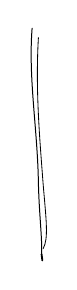
\begin{tikzpicture}[x=1cm,y=1cm,line cap=round]
\draw[line width=.36pt] (0,0) .. controls (-.05,-.64) and (.07,-1.29) .. (.08,-1.97)
 .. controls (.09,-2.38) and (.13,-2.67) .. (.12,-2.87);
\draw[line width=.30pt] (.08,-.12) .. controls (.04,-.79) and (.10,-1.44) .. (.14,-1.98)
 .. controls (.18,-2.45) and (.21,-2.67) .. (.14,-2.80);
\draw[line width=.65pt] (.12,-2.87) -- (.13,-2.95);
\end{tikzpicture}}}
\deleted{\unsure{$\operatorname{Hom}(K$}}
\[
 \unsure{\Gamma((X,S)/K)}\longrightarrow
 \begin{gathered}
 \text{Classes de $\pi$-conjugaison des}\\
 \text{sections de }\unsure{\mathcal E\to\Gamma}\text{ i.e.}\\
 \text{des sections de }\Pi_1(X)\to\Pi_1(e_K)
 \end{gathered}
\]

\margin{62}

\scanpage{64}
\mspage{30}

est bijective (si $(X,S)$ est un couple ``anabélien'').
\margin{faux tel quel, cf n° 9 ci-dessous --- il faut des conditions supplémentaires sur les $f$ \ldots\ \uline{\unsure{Peut-être}} \unsure{vrai si} $I=\varnothing$}

Je sais en tous cas que cette application est \uline{injective} --- ceci vaut chaque fois qu'on a un schéma $U$ sur $K$ (ici $X\setminus S$) qui se plonge dans un \inserted{groupe algébrique $G$,} extension d'une V.A. par un tore, et résulte alors du th. de Mordell-Weil ``absolu'': $G(K)$ est un $\mathbb Z$-module de type fini.
En fait, il suffit de connaître la classe de splittage de l'extension \unsure{$\mathcal E^\flat$|$\mathcal E^\sharp$} de $\Gamma$ par
\[
 \pi_{\mathrm{ab}}=\pi/\overline{[\pi,\pi]}\simeq H_1(\unsure{\mathrm{Alb}}),
\]
\deleted{\unsure{pour en déduire}} \inserted{correspondant} à un pt de $U$ rat/$K$, pour connaître ce point. Donc la \inserted{\unsure{totale}} fidélité est obtenue, sous des hyp. moins draconiennes sur $X$ que l'hyp. anabélienne (avec les notations \unsure{du numéro} \unsure{5.2|§2}, cela signifie que $g=0\Rightarrow\unsure{n|\nu}\ge2$ i.e. qu'il n'y a pas de comp. irréd. de \unsure{$X_{\overline K}$} qui soit isom. à \unsure{$\mathbb P^1_{\overline K}$} ou \unsure{$\mathbb E^1_{\overline K}$|$\mathbb A^1_{\overline K}$} \ldots).

\margin{63}

\scanpage{65}

\uline{NB} Ceci suggère une approche de la conjecture de Mordell, via une meilleure connaissance des extensions de $\Gamma$ par $\pi$: le fait qu'il n'y ait (pour $g\ge2$) qu'un nb fini de classes de $\pi$-conjugaison de scindages d'une telle extension \ldots.
Idem pour une approche du th. de Fermat, via \deleted{\illegible{1}} une bonne connaissance d'une extension de $\Gamma$ par $\pi=\pi_1(\unsure{\mathbb P^1_{\overline{\mathbb Q}}\setminus\{0,1,\infty\}})$ \ldots.

\uline{Cas $\overline{\mathrm{IV}}$} $n=1,n'=1$ i.e. $X,X'$ de dim 1.

a) Si $I=I'=\varnothing$, je n'ai rien à ajouter à la description des morphismes $f:X\to X'$ en termes de morphismes de diagrammes de groupoïdes. Ici \deleted{\illegible{1}} la condition $f^{-1}(S)_{\mathrm{r\acute ed}}=S'$ n'est pas une restriction sur $f$ --- \deleted{qui} on n'exclut donc pas des applications constantes. Celles-ci (grâce à
\margin{(\unsure{grâce à} \ldots)}
\deleted{Si \unsure{$I'\ne\varnothing$} \illegible{5} \unsure{seulement} $I'=\varnothing$ \inserted{\unsure{i.e. $S'=\varnothing$}} \illegible{7} \unsure{$S'$ est} \illegible{3} la condition}

\margin{64}

\scanpage{66}
\mspage{31}

l'étude du cas \uline{\unsure{$\overline{\mathrm{II}}$|$\overline{\mathrm{III}}$}}) sont d'ailleurs décrites de façon ``pleinement fidèle'' par des hom. de diagrammes --- Ils correspondent aux \unsure{cas} $f:\mathcal E'\to\mathcal E$ qui sont nuls sur $\pi'$.

b) Le cas $I'=\varnothing$, $I\ne\varnothing$ (i.e. $S'=\varnothing$, $S\ne\varnothing$) signifie, pour la condition $f^{-1}(S)_{\mathrm{r\acute ed}}=S'$ i.e. $f^{-1}(S)=\varnothing$, que $f$ doit appliquer $X'$ dans $X\setminus S$, \deleted{On s'attend donc} donc que les $f$ correspondant à un morphisme de $(X',\varnothing)$ dans $(X,S)$ sont constantes.
La conj. bordélique dans ce cas exprime donc \deleted{que} essentiellement qu'au niveau des hom. $\mathcal E'\xrightarrow{p'}\Gamma$ et $\mathcal E\xrightarrow{p}\Gamma$, tout hom. de groupes $\mathcal E'\xrightarrow{f}\mathcal E$ tel que $pf=\operatorname{int}(\alpha)p'$ pour $\alpha\in\Gamma$ [on est ramené au cas où $\alpha=1$, \inserted{$p,p'$ surjectifs} i.e. un hom d'extensions de $\Gamma$ par les gr-ps \unsure{$\pi=\pi_1(\overline{X\setminus S})$} et $\pi'=\pi_1(\overline{X'})$)] est trivial sur $\pi'$ [i.e. ``est'' une section]. Il faudrait essayer de vérifier ce point directement, qui (modulo le cas \uline{$\overline{\mathrm{III}}$}) établirait la ``conj. bordélique'' dans ce cas-là.

\margin{65}

\scanpage{67}

c) Le cas $I'\ne\varnothing$, $I=\varnothing$ implique que $\operatorname{Hom}((X,S),(X',S'))=\varnothing$ (car $f^{-1}(S)=f^{-1}(\varnothing)=\varnothing\ne S'$ !), ce qui correspond bien \deleted{au cas} à $\operatorname{Hom}(\mathcal D',\mathcal D)=\varnothing$ puisque $\nexists\tau:I'\to I$.

d) Dans le cas $I'\ne\varnothing$, $I\ne\varnothing$, la condition $f^{-1}(S)_{\mathrm{r\acute ed}}=S'$ implique que $f$ n'est pas constante (sinon on aurait $f^{-1}(S)_{\mathrm{r\acute ed}}=\varnothing$ ou $X'$), donc $f$ est dominant et fini, génériquement étale. [Donc, de telles $f$ ne \deleted{\unsure{sont admis} \illegible{1}} peuvent intervenir que si $I$ et $I'$ sont soit tous deux $\varnothing$ (cas a)), soit tous deux $\ne\varnothing$ (cas actuel d)). Le fait que dans ces cas là, la description \unsure{diagrammatique galoisienne} soit \uline{fidèle} (quoique pas pleinement) résulte aisément du résultat analogue dans le cas \uline{$\overline{\mathrm{III}}$}.
La pleine fidélité par contre est chose mystérieuse, $=$ si le résultat correspondant \deleted{\unsure{dans}} \deleted{\illegible{1}} au cas \uline{$\overline{\mathrm{III}}$} était acquis (\unsure{et on en}

\margin{66}

\scanpage{68}
\mspage{32}

semble loin, $=$ si $K$ fini sur $\mathbb Q$ \ldots)

\uline{Réductions} \uline{élémentaires} Pour prouver la ``conj. bordélique'', on est ramené (par des ext. finies des corps $K$) au cas où $\mathcal E\to\deleted{\unsure{K}}\Gamma$ (et, bien entendu, aussi $\mathcal E'\to\Gamma$) est épi. Sauf erreur, la connaissance du cas \uline{$\overline{\mathrm{III}}$} pour des extensions de t.f. de $K$, implique le cas général pour $K$ (avec possiblement des \unsure{menus truquages|ennuis techniques} \ldots).

Revenant cependant au cas général quand $\mathcal E\to\Gamma$ est surjectif, dans tte classe d'équival. de systèmes $(f:\mathcal E'\to\mathcal E,\alpha\in\Gamma,$ \deleted{\unsure{$f_i$,}} $\tau:I'\to I,$ \deleted{\unsure{$f_{i'}:\mathcal E'_{i'}$}} $(\alpha_{i'}\in\mathcal E_{\unsure{\tau(i')=i}})_{i'\in I'})$, on peut trouver un système avec $\alpha=1$, de sorte que $f:\mathcal E'\to\mathcal E$ est compatible avec les hom. dans $\Gamma$ (i.e. les structures d'extensions).
Quand on a deux de tels syst., leur équivalence par conjugaison se fait par un système \unsure{$(\mu,(\mu_{i'})_{i'\in I'})$} avec \uline{$\mu\in\pi$} $(=\operatorname{Ker}p)$, et

\margin{67}

\scanpage{69}

les $\mu_{i'}\in\mathcal E_{i=\tau(i')}$ comme avant. Ainsi, $f:\mathcal E'\to\mathcal E$ est \deleted{défini par des} \inserted{un} hom. d'extensions, défini aux autom. intérieurs par un élément de $\pi=\operatorname{Ker}(\mathcal E\to\Gamma)$, et satisfaisant des conditions explicitées par ailleurs.
Il se pourrait (comme on a déjà remarqué) que la connaissance de la classe de $\pi$-conj. de $f$ suffise à déterminer le ``morphisme bordélique'' dans lequel $f$ s'insère (si $I,I'\ne\varnothing$).

[C'est lié à la question de savoir si le \deleted{\illegible{2}} $\forall d\in\mathbb N^*,\ \operatorname{Trans}_{\mathcal E}(L_i^d,L_i)$ est réduit à $\mathcal E_i$ (où $L_i=\operatorname{Ker}(p_i:\mathcal E_i\to\Gamma)=\operatorname{Im}(\kappa_i:T(\overline K)\to\mathcal E_i)$).
\margin{\deleted{Il suffirait que \unsure{$\operatorname{Transp}(L_i^d,L_i)$} \illegible{2}}}
Dans ce cas, $\mathcal E_i$ serait connu en termes de $L_i\subset\pi$, et $=$ en termes du \unsure{rayon de ss-groupes} qu'il définit dans $\pi$, et a fortiori en termes du rayon d'hom. \unsure{défini} par $\kappa_i:T(\overline K)\to\pi$ \ldots.

\margin{68}

\scanpage{70}
\mspage{33}

\uline{Cas où} \inserted{les} $\mathcal E_i\to\Gamma$ est \uline{surjectif} (i.e. \inserted{les} \unsure{$k(s_i)=K$} i.e. $s_i$ rat. sur $K$).
Alors, si $(f,$ \deleted{\unsure{$\alpha$,}} $\tau,$ \deleted{\illegible{1}} $(\alpha_{i'}))$ est un hom de $\mathcal D'$ dans $\mathcal D$, \deleted{\illegible{2}} quitte à \deleted{\unsure{modifier}} \inserted{corriger} par des $\mu_i\in\mathcal E_i$ ayant $=$ image que les $\alpha_{i'}$ dans $\Gamma$, \unsure{OPS} $\alpha_{i'}\in\pi$, en plus de \unsure{$\alpha=1$} (obtenu en corrigeant par $\mu$ convenable).
Donc on décrit l'hom \inserted{$\mathcal D'\to\mathcal D$} par $(f,1,\tau,(\alpha_{i'}))$, les $\alpha_{i'}\in\pi$. Les \deleted{\unsure{systèmes}} \inserted{conditions} \deleted{\illegible{1}} sont que $f:\inserted{\mathcal E'\to\mathcal E}$ soit un hom. de groupes sur $\Gamma$, que \deleted{\unsure{$\operatorname{int}(\alpha_{i'}^{-1})$}} $f(\mathcal E'_{i'})\subset(\mathcal E_{\tau(i')=i})^{\unsure{\operatorname{int}(\alpha_{i'}^{-1})}}$, et que l'hom induit \inserted{$\mathcal E'_{i'}\to\mathcal E_i$} par \deleted{\unsure{$f_i=$}} \unsure{$\operatorname{int}(\alpha_{i'})f$|$\operatorname{int}(\alpha_{i'}^{-1})f$} \deleted{\unsure{de $\mathcal E_i$ de}} induit sur $T(\overline K)$ (\uline{via} $\kappa_{i'},\kappa_i$) \uline{l'hom de multiplication par $d_i$} sans plus --- que c'est beau!
Deux systèmes $(f,\tau,(\alpha_{i'}))$ et $(f',\tau',(\alpha'_{i'}))$ définissent le $=$ morphisme, \unsure{sss} \inserted{$\tau=\tau'$ et il} existe
\[
 \boxed{\mu\in\pi,\quad\mu_{i'}\in\unsure{L_{i=\tau(i')}|\mathcal E_{i=\tau(i')}}}
\]
\inserted{\unsure{$\kappa_i(T(\overline K))$}}
tels que
\[
 f'=\operatorname{int}(\mu)f
\]
\[
 \alpha'_{i'}=\mu_{i'}\alpha_{i'}.
\]

\deleted{\illegible{1}} Notons qu'à priori, pour $(f,\tau)$ fixé, les $\alpha_{i'}$ sont déterminés mod multiplication à droite par des éléments de
\[
 \operatorname{Transp}_{\pi}(\deleted{\unsure{\pi}}(\unsure{L_i^{d_{i'}}},L_i))
\]

\margin{69}
